\documentclass[BCOR20mm,DIV14,10pt,headinclude,footexclude,bibtotoc,liststotoc]{article}

\makeatletter
\author{Jonas Otto} \let\theauthor\@author
\newcommand\matrikelnr{982249}
\newcommand\topicNrTitle{4: Parallelization}
\newcommand\theWordCount{2.000-3.000}


% Satzspiegel {{{
\renewcommand{\baselinestretch}{1.10}
\setlength{\parindent}{0pt}
\setlength{\parskip}{10pt}
\setlength{\baselineskip}{0pt}
\widowpenalty10000
\clubpenalty10000
% }}}

\usepackage[utf8]{inputenc}
\usepackage[USenglish]{babel}

\usepackage{graphicx}
\usepackage[automark]{scrlayer-scrpage}

\usepackage{todonotes}
\presetkeys{todonotes}{inline}{}

\usepackage{hyperref}

\usepackage{amsmath}

\usepackage{cleveref}

\usepackage{pgfplots}
\pgfplotsset{compat=1.17}

% Make clickable footnote
\newcommand{\hyperfootnote}[1][]{\def\ArgI{{#1}}\hyperfootnoteRelay}
 % relay to new command to make extra optional command possible
 \newcommand\hyperfootnoteRelay[2][]{\href{#1#2}{\ArgI}\footnote{\href{#1#2}{#2}}}
 % the first optional argument is now in \ArgI, the second is in #1

\begin{document}
\begin{titlepage}

	
\includegraphics[height=1.8cm]{images/logo_100_sw_bildmarke}
	\hfill
	
\includegraphics[height=1.8cm]{images/logo_100_sw_wortmarke}\\[1em]


	{\footnotesize
	\hspace*{8.25cm}{\bfseries Fakult{\"a}t f{\"u}r\\
		\hspace*{8.25cm}Ingenieurwissenschaften\\
		\hspace*{8.25cm}und Informatik}\\
	\hspace*{8.25cm}Institut f{\"u}r Organisation und\\
	\hspace*{8.25cm}Management von Informations-
	\hspace*{8.25cm}systemen\\[1em]
	}

	\vspace{10em}
	\begin{center}
		\begin{Large}
			\topicNrTitle \\
		\end{Large}
		\vspace{15em}
		\theauthor \\
		Matrikelnummer: \matrikelnr \\
		ENGG 72323 - Heterogeneous and Parallel Computing Infrastructures \\
		Wordcount: \theWordCount
	\end{center}

\end{titlepage}

\section{Introduction}
%\subsection{Topic Description}
%Parallelization. Since the processor speed is hardly increasing anymore, the
%only way to really improve performance of an application is to parallelize.
%Discuss the different ways in which an application can be parallelized and why
%and when which method is preferable. Do all parallel applications scale well?
%Which factors determine the performance / scalability of an application and how
%can you affect them when writing the application.

In recent history, processor performance indicators such as frequency seem to
have stagnated. At the same time however, the number of processing cores in a
single system has steadily increased (\cref{fig:processor_trend}). This prompts
software developers to adopt a mindset of thinking about parallelization while
shaping today's software landscape, to keep up with advances in processor and
computer design.

Not all applications are suited to all forms of parallelism, and the scalability
and expected performance gain is finite. In this essay, the different ways in
which an application can be parallelized, and the factors determining
scalability, will be presented and discussed.

\begin{figure}[h]
	\centering
	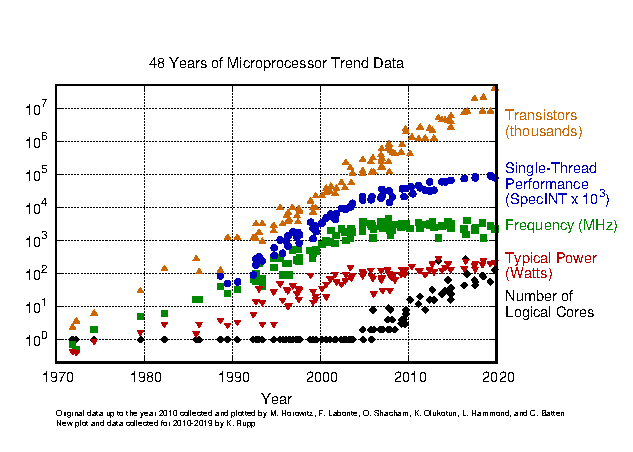
\includegraphics{images/48-years-processor-trend}
	\caption[48 Years of Microprocessor Trend Data]{
		\href{https://github.com/karlrupp/microprocessor-trend-data}
		{``48 Years of Microprocessor Trend Data''} by Karl Rupp, licensed under
		\href{https://creativecommons.org/licenses/by/4.0/}{CC BY 4.0}}
	\label{fig:processor_trend}
\end{figure}

\section{Analysis}

\subsection{Scalability: Amdahl's Law}

Given a program which contains some part that is not parallelizable
(sequential), a theoretical limit of speedup known as \emph{Amdahl's law}
can be determined:
\begin{description}
	\item[$s$] Fraction of purely sequential (non-parallelizable) code
	\item[$t$] Total execution time before parallelization
	\item[$n$] Number of cores/processors
\end{description}

This gives us a total execution time in the parallel case of:
\begin{equation}
	t_\text{parallel} = s \cdot t + \frac{(1-s)\cdot t}{n}
\end{equation}

Or a speedup of
\begin{eqnarray}
	\frac{t}{t_\text{parallel}} = \frac{n}{n \cdot s + (1-s)}
\end{eqnarray}

\begin{figure}
	\centering
	\begin{tikzpicture}
		\begin{axis}[
				width=\textwidth,
				height=0.5\textwidth,
				xmin=1, xmax=128,
				ymin=1, ymax=64,
				xtick={1,8,16,32,64,128},
				ytick={1,8,16,32,64},
				xlabel={Number of cores},
				ylabel={Speedup}
			]
			\foreach [evaluate=\s as \redfrac using (\s*10)] \s in {0,2,...,10} {
					\edef\temp{\noexpand\addplot[thick, domain=1:128, samples=200, red!\redfrac!green]{x/(x * (\s/100) + (1-(\s/100)))};
						\noexpand\addlegendentry{$s=\s\%$}}
					\temp
				}
		\end{axis}
	\end{tikzpicture}
	\caption{}
	\label{fig:amdahl}
\end{figure}

This provides us with a theoretical upper bound for the speedup we can expect
when parallelizing an application.


\subsection{Limitations of Amdahl's Law}
Amdahl's law provides an upper bound, but not one that a programmer can
reasonably expect to come close to. Even with trivially parallel problems, the
overhead induced by parallelizing is never zero. Communication, organization and
management of parallel execution threads takes time, and increases with the
number of threads. We expect to reach a point where the communication overhead
dominates the execution time compared to the actual application task. The
speedup decreases, and may even become negative, meaning the extra overhead
makes the parallel application run slower than the fully serial one.


\subsection{Task Parallelism}

In order to explore and model the ways in which an application can be
parallelized, two models are usually considered: Task- and data parallelism.

In this first part, the concept of task parallelism is explored. If an
application consists of multiple individual tasks, those can be performed
according to its dependencies. \Cref{fig:task_graph} illustrates this in terms
of a data flow graph: The individual tasks all require some input data, which is
provided by another task. It is however apparent that the tasks of creating a
grayscale image and then detecting the lane and the task of creating the RGB
image and detecting traffic signs can be executed in parallel. They both depend
on the camera image, but execute independently. The serial part of the
application continues with the tracking step, which depends on the results of
all the previous detection steps. Planning can only be performed after the
tracking step.

\begin{figure}
	\centering
	\begin{tikzpicture}
		\node[draw] (camera) {Camera};
		\node[draw] (grayscale) [right=of camera] {Bayer to grayscale};
		\node[draw] (lane) [right=of grayscale] {Detect lane};
		\node[draw] (rgb) [below=of camera] {Bayer to RGB};
		\node[draw] (signs) [right=of rgb] {Detect signs};
		\node[draw] (tracking) [right=of signs] {Tracking};
		\node[draw] (planning) [right=of tracking] {Planning};
		\node[draw] (viz) [below=of rgb] {Vizualization};
		\node[draw] (odom) [below=of tracking] {Odometry};

		\draw[->] (camera) -- (grayscale);
		\draw[->] (camera) -- (rgb);
		\draw[->] (grayscale) -- (lane);
		\draw[->] (lane) -- (tracking);
		\draw[->] (tracking) -- (planning);
		\draw[->] (rgb) -- (signs);
		\draw[->] (signs) -- (tracking);
		\draw[->] (rgb) -- (viz);
		\draw[->] (odom) -- (tracking);
	\end{tikzpicture}
	\caption{Data flow graph of a fictional task-parallel autonomous-driving application}
	\label{fig:task_graph}
\end{figure}

The \emph{critical path} is the path of execution that determines the execution
time of the entire application. 

\todo{critical path -> serial part (?)}

\todo{Dataflow/Dependency graphs}
\subsection{Data Parallelism}


\section{Discussion}

In the following, multiple ways of increasing the performance of an application
or system are considered. Special attention is given to methods which relieve
the programmer of some of the difficulties in programming a parallel
application, and still enable them to benefit from parallelization.

\todo{Patterns: https://www.stolaf.edu/people/rab/pdc/text/patterns.htm}

\todo{How can serial part of task be reduced or estimated?}
\todo{How are applications written? Retrofitting code with OpenMP?}

\subsection{Parallelism at application level}
\todo{Difficulties: manually using threading interfaces (pthreads), communication, synchronization, limitations such as GIL}
\todo{fork-and-join pattern}

\subsection{Parallelism below the application level}
\todo{Parallelism at lower levels? (Parallelizing low-level operations -> Libraries such as OpenCV)}
One solution to make programs more parallel without requiring the user (the
programmer) to manually implement parallel programming techniques, is to hide
the complexity in libraries below the application logic. One example is the
popular image processing library OpenCV: OpenCV hides complex algorithms behind
a relatively simple interface. Many of those algorithms in the field of image
processing lend themselves nicely to a data-parallel approach and benefit
greatly from parallelization. Therefore, OpenCV maintains a thread pool to
execute those operations, and even contains GPU implementations using OpenCL and
CUDA for some algorithms.

\subsection{Parallelism above the application level}
\todo{Parallelism at higher levels? (Executing multiple modules in parallel -> Frameworks such as ROS/ADTF, Microservices)}
A different approach to parallelizing application code which is not written in
an inherently parallel way is to exploit the fact that the application may
already be divided into more or less independent modules, which can be executed
in parallel. This is often the case, when the application code is embedded into
some kind of framework. The Robot Operating System ROS for example is a
framework popular for application in the fields of robotics and automation. A
core concept of this framework is the notion of a node, which is a program that
receives and publishes data via publish/subscribe channels and performs a
specific task (such as receiving sensor data or controlling actuators). Those
nodes can be started in individual processes (or threads), since they only rely
on the publish/subscribe communication channels for synchronization.

While this can lead to an immediate performance increase compared to serial
execution, this does not provide scalability with more processors. The upper
bound of performance increase is reached as soon as every node has enough
processing resource to not have to share them with another node (disregarding
the potential of each single node to benefit from multiple processors).

A similar effect can be achieved using MPI, which also provides an inter-process
communication channel and starts multiple processes, although in this case the
individual processes usually perform the same task on a smaller subset of data,
which enables greater scalability with the number of processes. This could be
considered an example for data parallelism, while the ROS example is closer to
task parallelism.

\section{Conclusion}

\cleardoublepage
\section*{Declaration of Originality}

I confirm that this assignment is my own work and that I have not sought or used
inadmissible help of third parties to produce this work and that I have clearly
referenced all sources used in the work. I have fully referenced and used
inverted commas for all text directly or indirectly quoted from a source.

This work has not yet been submitted to another examination institution –
neither in Germany nor outside Germany – neither in the same nor in a similar
way and has not yet been published.

\vspace{2cm}

Ulm, on the \dotfill

\hspace{10cm} {\footnotesize \theauthor}



\end{document}